\datos{color}{}{}
\subsection{\textit{RHex}}
\textit{RHex}, desarrollado inicialmente a comienzos de los años 2000 por un consorcio de
universidades liderado por la \textit{University of Michigan}, la \textit{University of Pennsylvania}
y \textit{McGill University}, Figura \ref{rhex}, es un robot hexápodo todoterreno diseñado para la
locomoción dinámica en terrenos irregulares. Su estructura ligera, su capacidad para desplazarse a
alta velocidad y su robustez mecánica lo convirtieron en una referencia en el estudio de la 
locomoción con patas y en el desarrollo de arquitecturas de control distribuidas y reactivas. 
\textit{RHex} emplea seis patas semirrígidas accionadas de manera independiente, lo que le permite 
correr, trepar, superar obstáculos y mantener la estabilidad incluso en superficies complejas. \\

Sus usos principales incluyen la investigación en locomoción bioinspirada, el estudio de
controladores reactivos, la exploración de terrenos no estructurados y el desarrollo de 
algoritmos de comportamiento distribuido. \textit{RHex} ha sido ampliamente utilizado en experimentos 
de campo, pruebas de movilidad extrema y estudios sobre estabilidad dinámica en robots de patas. \\

A diferencia de robots deliberativos clásicos como \textit{Shakey} o \textit{TurtleBot 4}, 
la arquitectura de \textit{RHex} es distribuida y se basa en la descomposición horizontal del 
problema. 
Cada pata dispone de controladores locales que procesan directamente la información sensorial 
y generan acciones motoras sin necesidad de un planificador central. Los módulos siguen
el principio de niveles de competencia: los controladores 
básicos garantizan la estabilidad y la locomoción elemental, mientras que capas superiores 
añaden comportamientos como evitar obstáculos, trepar o ajustar la postura. El comportamiento 
global del robot emerge de la interacción entre estos módulos, lo que permite respuestas rápidas y 
adaptativas ante cambios del entorno.\\

\begin{wrapfigure}{r}{0.34\textwidth}
    \centering
    \vspace{-10pt}
    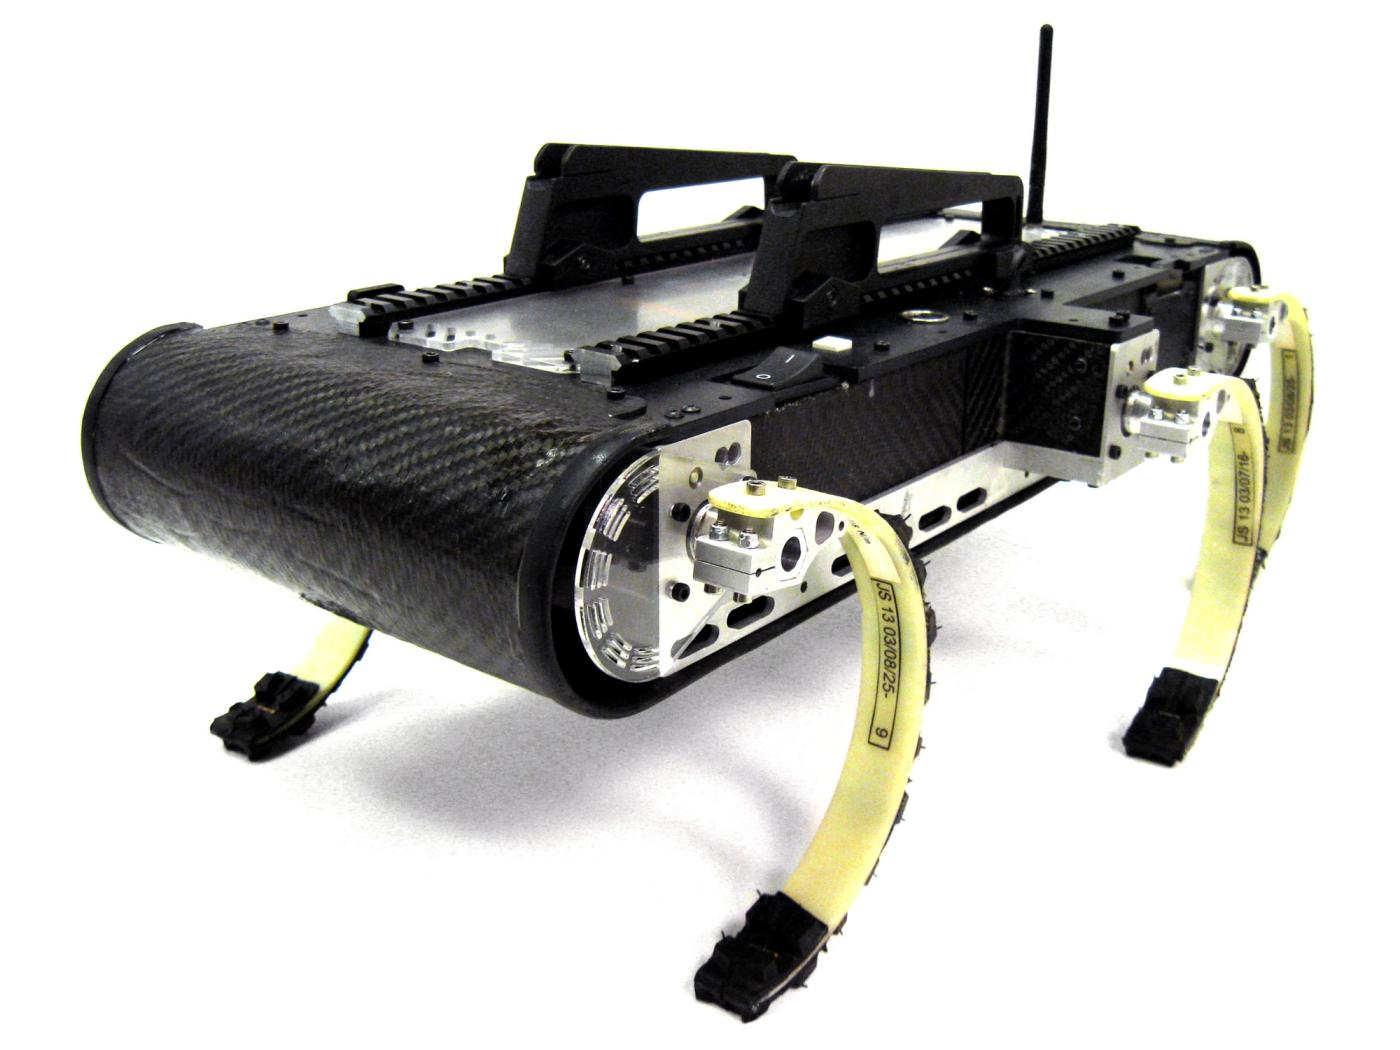
\includegraphics[width=0.34\textwidth]{Images/rhex.jpg}
    \caption{\label{rhex}\textit{RHex}.}
    \vspace{-10pt}
\end{wrapfigure}

\textit{RHex} utiliza un sistema de locomoción basado en seis patas rotatorias elásticas, 
cada una accionada por un motor independiente. La forma semicircular de las patas y su 
flexibilidad permiten generar tracción continua y absorber irregularidades del terreno. 
Variando la velocidad y fase relativa de las patas, el robot puede avanzar, girar, estabilizarse 
y ejecutar maniobras dinámicas como saltos o ascensos por superficies inclinadas. Este diseño 
mecánico, combinado con controladores distribuidos, le proporciona una movilidad excepcional 
en entornos donde los robots con ruedas o cadenas tienen dificultades. \\

\subsection*{Referencias}
\cite{doi:10.1177/02783640122067570} \fullcite{doi:10.1177/02783640122067570}.